% Chapter 5 - Results

\glsresetall % reset the glossary to expand acronyms again
\chapter[Results]{Results}\label{ch:Results}
\index{Results}

% Results
\section[Results]{Results}
\begin{itemize}
	\item{Describe the experimental setup (ie. Hardware)}
	\item{Describe your experiments}
	\item{Describe your results}
\end{itemize}

This chapter should generally present your finding in the form of figures, tables, equations, code listings, etc. It is for presenting and discussing your findings, which can split into sections if the experiment has multiple parts, or stages.  You might also want to have a `Discussion' or `Discussion of Results' chapter, which may focus on either more detailed discussion of particular results, or more comprehensive discussion of the results and system performance as a whole.  If you have a Discussion of Results section, then you do not want to discuss too much about the specific results in this chapter and rather move the main discussion or reflective considerations of these to the Discussion of Results chapter.

However, and this is an important reminder, ensure that you do have some text of discussion for your results, to take the reader through your results and the figures you may provide.  Make sure not to just put one figure after another without any attempt to explain the sequencing and what is being shown and perhaps some key issues in the figures presented (a monolithic sequence of figure after figure without any attempt at explanation will get undesirable responses from examiners).

If you have an experiments section, it is often useful to have a clear connection of experiment section corresponding to a result section showing results for that test. Examiners often appreciate that sort of clear and consistent structure that is easy to follow.  For example, if you have section~5.1 as Modular Testing, then you could correspond to~6.1 Modular Testing Results (the two sections should be cross-linked with \verb|\label| and \verb|\ref|, in both directions)

\section{Tips for Results Figures}

Include good quality graphs (see Fig.~\ref{fig:r_vs_N_f=0_0005_P=90} for an example).

\begin{figure}[ht]
\centering
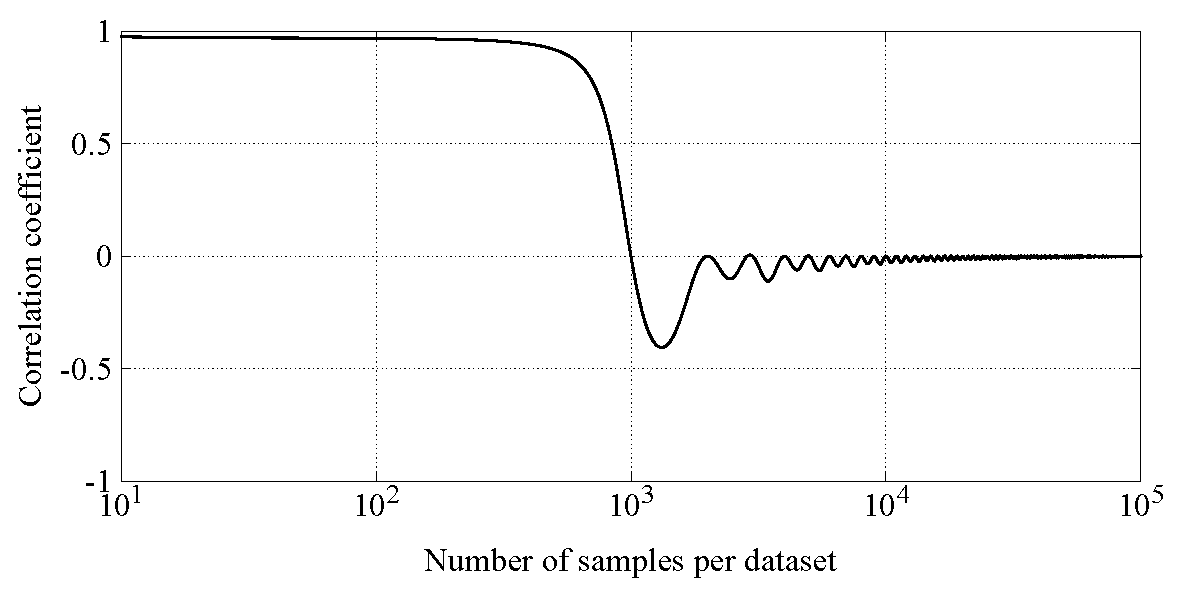
\includegraphics[width=0.8\columnwidth]{3_Chapters/5_Chapter_Results/Figures/r_vs_N_f=0_0005_P=90.pdf}
\caption{The correlation coefficient as a function of sample count}
\label{fig:r_vs_N_f=0_0005_P=90}
\end{figure}

An easy way to obtain more space for an article is to use wide, flat figures, such as Fig.~\ref{fig:Line_Signals}.

\begin{figure}[ht]
\centering
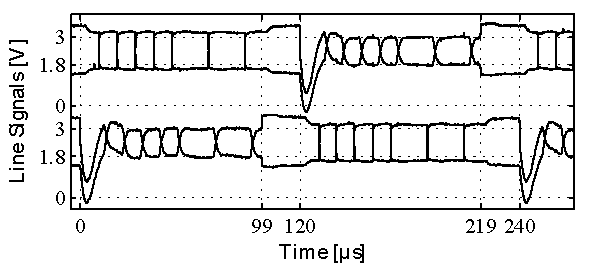
\includegraphics[width=0.8\columnwidth]{3_Chapters/5_Chapter_Results/Figures/Line_Signals.pdf}
\caption{Oscilloscope measurement showing physical line signals on both ends of a transmission line during master switch-over~\cite{Taylor_2016}}
\label{fig:Line_Signals}
\end{figure}


\section{Pictures and screenshots}

When you include screenshots, pdf\LaTeX{} supports JPG and PNG file formats.  PNG is preferred for screenshots, as it is a loss-less format.  JPG is preferred for photos, as it results in a smaller file size.  It's generally a good idea to resize photos (not screenshots) to be no more that 300~dpi, in order to reduce file size. \textbf{Never change the aspect ratio of screenshots and pictures!}

Fig.~\ref{fig:UCT.pdf} shows an example of a PDF image with custom scaling.

\begin{figure}[ht]
\centering

\includegraphics[width=0.35\columnwidth]{3_Chapters/5_Chapter_Results/Figures/UCT.pdf}
\caption{An example image with custom scaling}
\label{fig:UCT.pdf}
\end{figure}

Make sure to always use the best quality image possible.  Use JPEG for photos, PNG for screenshots and PDF (scalable vector graphics) for everything else.  JPEG is lossy, but good for photos, whereas PNG is lossless and good for images with large areas of solid colour.\\

\vspace{5mm}
\hfill
\begin{minipage}[b]{0.3\textwidth}\centering\setlength{\parindent}{0mm}

\includegraphics[width=\textwidth]{3_Chapters/5_Chapter_Results/Figures/UCT.jpg}\\%
{\small (a)~~JPEG}%
\end{minipage}
\hfill
\begin{minipage}[b]{0.3\textwidth}\centering\setlength{\parindent}{0mm}

\includegraphics[width=\textwidth]{3_Chapters/5_Chapter_Results/Figures/UCT.png}\\%
{\small (b)~~PNG}%
\end{minipage}
\hfill
\begin{minipage}[b]{0.3\textwidth}\centering\setlength{\parindent}{0mm}

\includegraphics[width=\textwidth]{3_Chapters/5_Chapter_Results/Figures/UCT.pdf}\\%
{\small (c)~~SVG}%
\end{minipage}
\hfill\mbox{}

